\chapter{Ottimizzazione con le Reti Neurali} % (fold)
\label{cha:ottimizzazione_con_le_reti_neurali}
In questo capitolo si analizza l'utilizzo di una rete di Hopfield, come strumento di ottimizzazzione, per fornire una soluzione ottimale a problemi NP-Difficile. In particolare sarà introdotto il problema del commesso viaggiatore (Traveling Salesman Problem).

\section{Problema del commesso viaggiatore} % (fold)
\label{sec:problema_del_commesso_viaggiatore}
In questa sezione si introduce il problema del commesso viaggiatore (abbreviato TSP) e una sua possibile soluzione attraverso l'utilizzo delle reti di Hopfield.\\

Il nome del problema nasce dalla sua più tipica rappresentazione: data una rete di città, connesse tramite delle strade, trovare il percorso di minore lunghezza che un commesso viaggiatore deve seguire per visitare tutte le città una e una sola volta per poi tornare alla città di partenza.\\

Il problema è di considerevole importanza pratica, al di là delle ovvie applicazioni nella logistica e nei trasporti. Un esempio classico è la costruzione di circuiti stampati, nella pianificazione del percorso del trapano per creare i fori nella piastra.


\subsection{Formulazione del problema} % (fold)
\label{sub:formulazione_del_problema}
Espresso nei termini della teoria dei grafi il TSP è così formulato: \emph{dato un grafo completo pesato $G=(V, E, w)$, trovare il cammino di costo minore visitando tutti i nodi $V$ una sola volta e tornando al nodo di partenza.}\\

La rete di città può essere rappresentata come un grafo in cui le città sono i nodi $V$, le strade gli archi $E$ e le distanze i pesi sugli archi $w$. La differenza sostanziale rispetto al Ciclo Hamiltoniano si trova nel fatto che quest'ultimo è formulato su di un grafo privo di pesi. Il problema è NP-completo: per poter trovare il percorso minimo è necessario elencare tutti gli \textbf{$n!$} percorsi.

\newpage

\begin{figure}[h!]
    \centering
    \begin{tikzpicture}
        
        \node[circle,fill=blue!20] (A) at (0,2) {A};
        \node[circle,fill=blue!20] (B) at (-2,0) {B};
        \node[circle,fill=blue!20] (C) at (2,0) {C};
        \node[circle,fill=blue!20] (D) at (0, -2) {D};
        
        \foreach \from / \to in {B/A,B/D}
            \path (\from) edge[left] node {$w_{\from\to}$} (\to);
        
        \foreach \from / \to in {C/A,C/D}
             \path (\from) edge[right] node {$w_{\from\to}$} (\to);
             
         \path (A) edge[below left=0.1cm  of A] node {$w_{AD}$} (D);
         \path (B) edge[above right=0.1cm  of C] node {$w_{BC}$} (C);
             
    \end{tikzpicture}
    \caption{Grafo completo pesato.}\label{fig:graph}
\end{figure}

% subsection formulazione_del_problema (end)

\subsection{Soluzione del TSP con le reti di Hopfield} % (fold)
\label{sub:soluzione_del_tsp_con_le_reti_di_hopfield}
Risolvere un problema di ottimizzazione con le reti di Hopfield richiede di \emph{trovare una funzione di energia $E$ adeguata in modo tale che il minimo corrisponda alla soluzione del problema che si sta affrontando.}\\

Per prima cosa è necessario rappresentare il TSP attraverso una matrice di permutazione per identificare un percorso. Ad esempio dato il grafo in Figura~\ref{fig:graph}, il percorso $B \rightarrow A \rightarrow C \rightarrow D$ può essere rappresentato con la seguente matrice:\\

\begin{table}[h!]
    \centering
    \begin{tabularx}{8cm}{lXXXX}
        \toprule
        \backslashbox{Città}{Fermata} & 1 & 2 & 3 & 4 \\
        \midrule
        A & 0 & \textbf{1} & 0 & 0 \\
        B & \textbf{1} & 0 & 0 & 0 \\
        C & 0 & 0 & \textbf{1} & 0 \\
        D & 0 & 0 & 0 & \textbf{1} \\
        \bottomrule
    \end{tabularx}
    \caption{Matrice di permutazione del percorso BACD}
\end{table}

Dunque per $n$ città saranno necessari $n \times n$ neuroni nella rete di Hopfield in cui ogni neurone identifica una città e una fermata.

\newpage

\begin{figure}[h!]
    \centering
    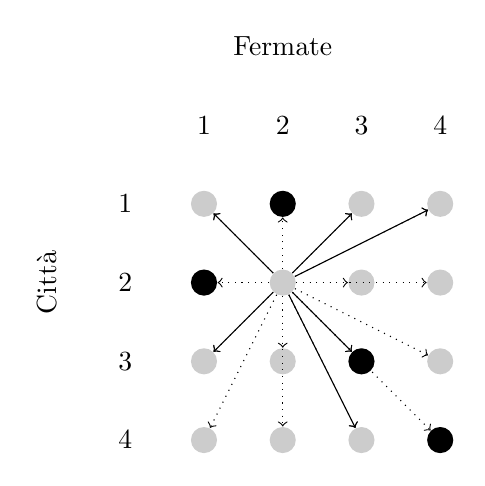
\begin{tikzpicture}
        
        \foreach \x / \y in {1/1,2/2,3/3,4/4} {
            \node (0-\x) at (0, -\x) {\y};
            \node (\x-0) at (\x, 0) {\x};
        }
        
        \foreach \x in {1,...,4} {
            \foreach \y in {1,...,4} 
                \node[circle, fill=black!20] (\x-\y) at (\x, -\y) {};
        }
        
        \foreach \x / \y in {1/1, 1/2, 1/3, 1/4, 2/1, 2/3, 2/4, 3/1, 3/2, 3/3, 3/4, 4/1, 4/2, 4/3, 4/4}
            \path (2-2) edge[dotted, ->] (\x-\y);
        
        \foreach \x / \y in {1/1, 1/3, 3/3,3/1, 3/4, 4/1}
            \path (2-2) edge[->] (\x-\y);
        
        \foreach \x / \y in {1/2, 2/1, 3/3, 4/4} {
            \node[circle, fill=black] at (\x,-\y) {};
        }
        
        \node[above of=2-0] {Fermate};
        \node[left of=0-2, rotate=90] {Città};
        
    \end{tikzpicture}
    \caption{Rappresentazione di una rete di Hopfield in un TSP con quattro città $n=4$. I punti neri indicano le unità attive $=1$ quando la rete sta rappresentando il percorso $3 \rightarrow 2 \rightarrow 4 \rightarrow 1$. Le connessioni sono mostrate solo per l'unità $n_{22}$. Linee solide indicano connessioni inibitorie di forza $- d_{ij}$, mentre linee tratteggiate sono connessioni inibitorie uniformi di forza $-Y$. Tutte le connessioni sono simmetriche.} 
\end{figure}

La soluzione del problema sarà dunque una matrice $V$ di dimensione $n \times n$. Si introducono ora alcune notazioni:
\begin{itemize}
    \item $X$ indica la città;
    \item $i$ una fermata in cui è visitata una città;
    \item $V_{X,i}$ è l'output dell'unità $X, i$;
    \item $T_{Xi, Yj}$ sono i pesi delle connessioni;
    \item $V_{X,i} = 1$ se la città $X$ è visitata alla fermata $i$;
    \item $d_{X,Y}$ distanza tra la città $X$ e $Y$.
\end{itemize}

Si definisce ora la funzione obiettivo da minimizzare che rappresenta il costo totale del cammino:
\begin{align*}
    E_1  = \frac{D}{2} \sum_X \sum_{Y \neq X} \sum_i d_{X,Y} V_{X,i} (V_{Y, i-1} + V_{Y, i+1})
\end{align*}
dove $D$ è una costante e gli indici sono intesi modulo $n$. La matrice $V$ senza vincoli di alcun genere può descrivere zero o più percorsi di lunghezza arbitraria (quindi può anche non toccare tutte le città).
Se la matrice $V$ descrivesse solo percorsi unici Hamiltoniani, allora minimizzando la funzione costo $E_1$ otterremmo la soluzione. Tuttavia il problema del commesso viaggiatore presenta una serie di \textbf{vincoli} che devono essere rispettati dalla matrice $V$.

\newpage


\begin{figure}[h!]
    \centering
    
    \subfigure{
    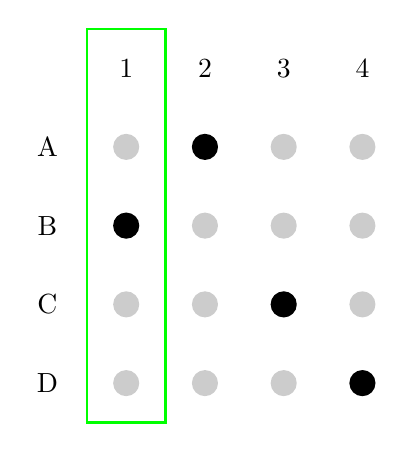
\begin{tikzpicture}
        
        \foreach \x / \y in {1/A,2/B,3/C,4/D} {
            \node (0-\x) at (0, -\x) {\y};
            \node (\x-0) at (\x, 0) {\x};
        }
        
        \foreach \x in {1,...,4} {
            \foreach \y in {1,...,4} 
                \node[circle, fill=black!20] (\x-\y) at (\x, -\y) {};
        }

        \foreach \x / \y in {1/2, 2/1, 3/3, 4/4} {
            \node[circle, fill=black] at (\x,-\y) {};
        }
        
        \draw[green, thick] (0.5,0.5) rectangle (1.5,-4.5);
        
    \end{tikzpicture}}
    \qquad
    \subfigure{
    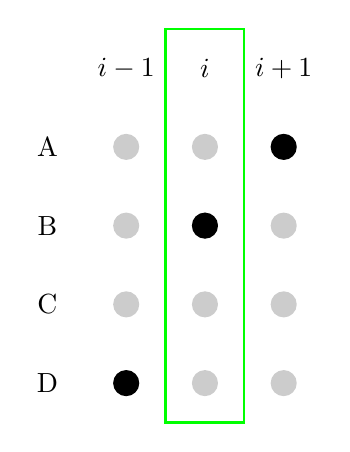
\begin{tikzpicture}
        \foreach \x / \y in {1/A,2/B,3/C,4/D}
            \node (0-\x) at (0, -\x) {\y};
        
        \foreach \x / \y in {1/$i-1$, 2/$i$, 3/$i+1$}
            \node (\x-0) at (\x, 0) {\y};
        
        \foreach \x in {1,...,3}
            \foreach \y in {1,...,4} 
                \node[circle, fill=black!20] at (\x, -\y) {}; 
                
        \foreach \x / \y in {4/1, 2/2, 1/3} {
            \node[circle, fill=black] at (\y,-\x) {};
        
        \draw[green, thick] (1.5,0.5) rectangle (2.5,-4.5);
        }
    \end{tikzpicture}}
    \caption{Interpretazione grafica di $E_1$}
\end{figure}

Di seguito si riportano i vincoli per il TSP:

\begin{enumerate}
    \item \textbf{Vincolo sulle righe}: Ogni città deve essere visitata una sola volta. Ovvero le righe della matrice $V$ devono avere soltanto un elemento impostato ad 1, il resto a 0;
    \begin{align*}
        E_2 = \frac{A}{2} \sum_X \sum_i \sum_{j \neq i} V_{X,i} V_{X,j}
    \end{align*}
    che vale 0 (il minimo) se ogni città è visitata al massimo una volta.
    \item \textbf{Vincolo sulle colonne}: Ogni fermata deve contenere una città, ovvero ogni colonna della matrice $V$ abbia un elemento impostato ad 1 ed il resto a 0;
    \begin{align*}
        E_3 = \frac{B}{2} \sum_i \sum_X \sum_{Y \neq X} V_{X,i} V_{Y,i}
    \end{align*}
    che vale 0 se ogni step del tour contiene al massimo una città.
    \item \textbf{Vincolo sulle entrate}: in totale devono essere attraversate $n$ città.
    \begin{align*}
        E_4 = \frac{C}{2}\left(\sum_X \sum_i V_{X,i} - n \right)^2
    \end{align*}
    che vale 0 se il numero di città attraversate è esattamente $n$.
\end{enumerate}

\newpage

Ci si trova dunque con quattro funzioni energia da minimizzare, tuttavia per poter utilizzare una rete di Hopfield è necessaria un'unica funzione. Per questo motivo si esprime la funzione costo totale come combinazione lineare delle funzioni energia $E_i$:
\begin{align}
    E = E_1 + E_2 + E_3 + E_4
\end{align}
dove il peso da attribuire a ciascun termine è determinato dalle costanti positive $A, B, C, D$. La funzione energia risultante dovrà essere della forma tipica di una rete di Hopfield ovvero nella forma dell'Equazione~\eqref{eq:energy}:
\begin{align*}
     E = - \frac{1}{2} \sum_{X, Y} \sum_{i, j} T_{X_i, Y_j} V_{X_i} V_{Y_j} - \sum_{X_i} I_{X_i} V_{X_i}
\end{align*}
Per ricondursi alla funzione energia tipica di Hopfield si utilizza un “trucco”: si introduce il seguente termine:
\begin{align*}
	\delta_{i,j} =
	\begin{cases}
		1, &\text{ se } i = j\\
		0, &\text{ se } i \neq j \\
	\end{cases}
\end{align*}
Le funzioni energia si possono ora riscrivere nel seguente modo:
\begin{align*}
	E_1 &= \frac{D}{2} \sum_X \sum_{Y \neq X} \sum_i d_{X,Y} V_{X,i} (V_{Y, i+1} + V_{Y, i-1}) \\
	&=  \frac{D}{2} \sum_{X,Y} \sum_{i,j} d_{X,Y} V_{X,i} V_{Y,j} \cdot (\delta_{j, i-1} + \delta_{j, i+1})
\end{align*}

\begin{align*}
    E_2 &= \frac{A}{2} \sum_X \sum_i \sum_{j \neq i} V_{X,i} V_{X,j} \\
	&= \frac{A}{2} \sum_{X,Y} \sum_{i,j} V_{X,i} V_{Y,j} \delta_{X,Y} (1 - \delta_{i,j})
\end{align*}

\begin{align*}
    E_3 &= \frac{B}{2} \sum_i \sum_X \sum_{Y \neq X} V_{X,i} V_{Y,i} \\
	&= \frac{B}{2} \sum_{X,Y} \sum_{i,j} V_{X,i} V_{Y,j} \delta_{i,j} (1 - \delta_{X,Y})
\end{align*}

\begin{align*}
    E_4 &= \frac{C}{2}\left(\sum_X \sum_i V_{X,i} - n \right)^2 \\
	&= \frac{C}{2} \left(\left(\sum_X \sum_i V_{X,i}\right)^2 - 2n \cdot \sum_X \sum_i V_{X,i} + n^2 \right)
\end{align*}
dove
\begin{align*}
	\left(\sum_X \sum_i V_{X,i}\right)^2 &= \left(\sum_X \sum_i V_{X,i}\right) \cdot \left(\sum_X \sum_i V_{X,i} \right) \\
	&= \sum_{X,Y} \sum_{i,j} V_{X,i} V_{Y,j}
\end{align*}
In $E_4$ il termine costante $n^2$ si può tralasciare, in quanto non modifica il punto in cui si ottiene il minimo, ma il valore della funzione $E_4$ in corrispondenza del minimo.
Mettendo il tutto assieme si ottiene la \textbf{funzione di energia totale}:
\begin{align*}
	E &= \frac{A}{2} \sum_{X,Y} \sum_{i,j} V_{X,i} V_{Y,j} \delta_{X,Y} (1 - \delta_{i,j}) \\
	&+ \frac{B}{2} \sum_{X,Y} \sum_{i,j} V_{X,i} V_{Y,j} \delta_{i,j} (1 - \delta_{X,Y}) \\
	&+ \frac{C}{2} \left(\sum_{X,Y} \sum_{i,j} V_{X,i} V_{Y,j} - \sum_{X,i} V_{X,i} \right) \\
	&+ \frac{D}{2} \sum_{X,Y} \sum_{i,j} d_{X,Y} V_{X,i} V_{Y,j} \cdot (\delta_{j, i-1} + \delta_{j, i+1}) \\
	&= - \frac{1}{2} \sum_{X, Y} \sum_{i, j} T_{X_i, Y_j} V_{X_i} V_{Y_j} - \sum_{X_i} I_{X_i} V_{X_i}
\end{align*}
Dove $T_{Xi, Yj}$ sono i pesi che la rete deve scoprire:
\begin{align*}
	T_{Xi, Yj} &= - A \delta_{XY} (1 - \delta_{ij}) \tag{peso inibitorio in ogni riga}\\
	& - B \delta_{ij} (1 - \delta_{XY}) \tag{peso inibitorio in ogni colonna} \\
	& - C  \qquad \tag{Inibizione globale}\\
	& - D d_{XY} (\delta_{j,i-1} + \delta_{j, i+1}) \tag{Termine dei dati}
\end{align*}
e il vettore di corrente esterna $I$ ha come $Xi$-esima componente:
\begin{align*}
	I_{Xi} = C_n \tag{Corrente esterna eccitatoria}
\end{align*}
% subsection soluzione_del_tsp_con_le_reti_di_hopfield (end)

\newpage

\subsection{Un'altra formulazione} % (fold)
\label{sub:un_altra_formulazione}
La determinazione dei parametri $A, B, C, D$ è particolarmente difficile. Pertanto un altro modo per esprimere i vincoli del TSP (cioè la matrice di permutazione $V$) è il seguente:
\begin{align*}
	E_2 = \frac{A}{2} \sum_X \left(\sum_i V_{X, i} - 1 \right) ^ 2 \tag{Vincolo sulle righe} \\
	E_3 = \frac{B}{2} \sum_i \left(\sum_X V_{X, i} - 1 \right) ^ 2 \tag{Vincolo sulle colonne} \\
\end{align*}
Quindi la funzione energia diventa:
\begin{align*}
	E = \frac{D}{2} \sum_{X} \sum_{Y \neq X} \sum_i d_{X,Y} V_{X,i}(V_{Y, i + 1} + V_{Y, i - 1}) + E_2 + E_3
\end{align*}
Dal momento che $E_4$ non è usato abbiamo tre parametri anziché quattro.
% subsection un_altra_formulazione (end)


\subsection{Problema delle n regine} % (fold)
\label{sub:problema_delle_n_regine}
Una famosa variante del TSP è il \emph{problema delle n regine}. Si immagini una scacchiera $n \times n$ e $n$ regine; una regina può muoversi lungo le righe, le colonne e le diagonali. Il problema consiste nel posizionare questi $n$ pezzi in modo tale che nessuno di essi possa attaccarsi l'uno contro l'altro.\\

Si può costruire una rete di Hopfield $n \times n$ in cui il neurone $(i,j)$ è attivo se e solo se una regina occupa la posizione $(i,j)$. Ci sono inoltre quattro vincoli:
\begin{enumerate}
    \item solo una regina in ciascuna riga;
    \item solo una regina in ciascuna colonna;
    \item solo una regina in ciascuna diagonale;
    \item solo $n$ regine sulla scacchiera.
\end{enumerate}

\newpage

Il problema è analogo al TSP con l'aggiunta del vincolo sulle diagonali. La matrice dei pesi è quindi data da:
\begin{align*}
	- T_{ij,kl} &= - A \delta_{ik} (1 - \delta_{ij}) \tag{peso inibitorio in ogni riga}\\
	& + B \delta_{jl} (1 - \delta_{ik}) \tag{peso inibitorio in ogni colonna} \\
	& + C  \qquad \tag{Inibizione globale}\\
	& + D (\delta_{i+j,k-l} + \delta_{i-j, k-l})(1 - \delta_{ik}) \tag{peso inibitorio sulle diagonale}
\end{align*}
% subsection problema_delle_n_regine (end)
% section problema_del_commesso_viaggiatore (end)

\newpage

\section{Problema della cricca massima} % (fold)
\label{sec:problema_della_cricca_massima}

Sia $G=(V,E)$ un grafo non orientato con $V$ l'insieme dei vertici ed $E$ quello degli archi, tale per cui $V={1,\dots,n}$ e $E \subseteq V \times V$. Si definisce cricca (o clique) $C \subseteq V$, un sottoinsieme di vertici di G mutuamente adiacenti (che formano un grafo completo), ovvero tali che $\forall i,j \in C$ con $i \neq j, (i,j) \in E$.

\begin{mydef}[Clique massimale]
Si definisce \textbf{clique massimale} di $G$ una clique di $G$ che non è contenuta in nessun'altra clique di $G$.    
\end{mydef}

\begin{mydef}[Clique massima]
    Si definisce \textbf{clique massima} di $G$ una clique massimale di G di cardinalità massima.
\end{mydef}
Il problema consiste nel trovare una cricca massimale (MCP). Ad esempio si consideri il seguente grafo:

\begin{figure}[h!]
    \centering
    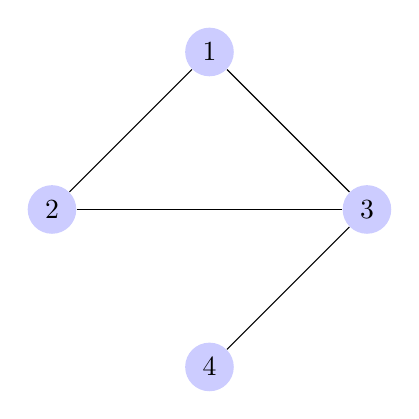
\begin{tikzpicture}
        \node[circle,fill=blue!20] (1) at (0,2) {1};
        \node[circle,fill=blue!20] (2) at (-2,0) {2};
        \node[circle,fill=blue!20] (3) at (2,0) {3};
        \node[circle,fill=blue!20] (4) at (0, -2) {4};
    
        \foreach \from / \to in {1/2,2/3,1/3,3/4}
            \path (\from) edge (\to);
    \end{tikzpicture}
    \caption{Un grafo non orientato.}\label{fig:graph1}
\end{figure}
Le clique nel grafo sono:
\begin{align*}
    C_1 &= \{1,2\} \tag{$C_1$ non è massimale perché $C_1 \subseteq C_2$}\\
    C_2 &= \{1,2,3\} \tag{Massimale e massima}\\
    C_3 &= \{3,4\} \tag{Massimale}
\end{align*}

\newpage

Trovare la cricca massimale è un problema facile, mentre trovare quella massima è NP-difficile, così come trovare la dimensione di tale clique. In questa sezione si affronta il problema sotto quest'ultimo punto di vista.

\subsection{Formulazione continua di MCP} % (fold)
Per affrontare il problema con le reti neurali è necessario trasformare MCP da problema discreto a problema continuo. Nell'esempio del TSP con il modello di Hopfield, non è detto che ci sia il percorso inverso (potremo ottenere ad esempio una matrice che non ha significato); in questo nuovo problema MCP, la bidirezionalità è d'obbligo.\\

Si utilizza quindi un nuovo approccio, ma prima sono necessarie alcune notazioni:
\begin{itemize}
    \item Se $C \subseteq V$, $x^C$ indica il \textbf{vettore caratteristico} definito come:
    \begin{align*}
        x^C_i = 
        \begin{cases}
            \displaystyle\frac{1}{|C|}, &\text{se }i \in C\\
            0,  &\text {altrimenti}
        \end{cases}
    \end{align*}
    dove $|C|$ indica la cardinalità dell'insieme $C$ e $i \in \{ 1, \dots, |V|\}$
    \item $S_n$ è il \textbf{simplesso standard} in $\mathbb{R}^n$:
    \begin{align*}
        S_n = \left\{x \in \mathbb{R}^n : \sum_{i=1}^n x_i = 1 \text{ e } x_i \geq 0, \forall i \right\}
    \end{align*}
    Per qualunque vettore caratteristico vale la relazione $x^C \in S_n$ con $n \geq |C|$
    \item $A=(a_{ij})$ è la matrice di adiacenza di $G$:
    \begin{align*}
        a_{ij} =
        \begin{cases}
            1, &\text{ se } (i,j) \in E \\
            0, &\text{ altrimenti}
        \end{cases}
    \end{align*}
\end{itemize}

\newpage

\begin{figure}[h!]
    \centering
    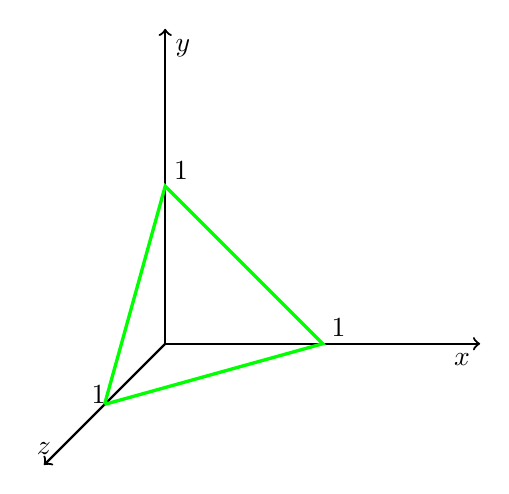
\begin{tikzpicture}[scale=2]

        %draw the main coordinate system axes
        \draw[thick,->] (0,0,0) -- (2,0,0) node[anchor=north east]{$x$};
        \draw[thick,->] (0,0,0) -- (0,2,0) node[anchor=north west]{$y$};
        \draw[thick,->] (0,0,0) -- (0,0,2) node[anchor=south]{$z$};
        
        \draw[thick, color=green, very thick] plot coordinates{(0,0,1) (0,1,0) (1,0,0) (0,0,1)};
        
        \node at (1.1,0.1,0) {1};
        \node at (0.1,1.1,0) {1};
        \node at (0,0.1,1.1) {1};
        
    \end{tikzpicture}
    \caption{Rappresentazione grafica del simplesso standard}
\end{figure}

Si consideri la seguente funzione quadratica continua in $n$ variabili:
\begin{align*}
    &f_G(x) = x^T A x = \sum_{i=1}^n \sum_{j=1}^n a_{ij} x_i x_j \tag{Lagrangiano del grafo} \\
    &\text{oppure } f_G(\bar{x}) = \sum_{(i,j) \in E} x_i x_j
\end{align*}
dove $x^T$ è il vettore trasposto e $A$ è la matrice di adiacenza. Ad esempio se si considera il grafo in Figura~\ref{fig:graph1} allora:
\begin{align*}
    f_G(x) = x_1 x_2 + x_1 x_3 + x_2 x_3 + x_3 x_4
\end{align*}

È stata dunque definita una funzione continua che rappresenta il problema: il Lagrangiano del grafo. A questo punto l'approccio tipico per risolvere MCP è quello di costruire un sistema dinamico che converga ai massimi di tale funzione. Questi punti corrisponderanno alle soluzioni nello spazio discreto del problema originale. A tale scopo si introduce il teorema di Motzkin-Strauss.
\begin{thm}[Teorema di Motzkin-Strauss]
    Sia $x^*$ un massimo globale di $f_G$ in $x \in S_n$ allora la cardinalità della clique massima è legata a $f_G(x)$  dalla seguente formula:
    \begin{align*}
           \omega(G) = \frac{1}{1 - f(x^*)}
    \end{align*}
    Inoltre un sottoinsieme di vertici $C$ è una clique massima se e solo se il suo vettore caratteristico $x^C \in S_n$ è un massimo globale per $f_G$ in $S_n$.
\end{thm} 
\newpage

Il teorema di Motzkin-Strauss fornisce una connessione tra la cardinalità della clique massima $\omega(G)$ di un grafo $G$ con $n$ vertici e il massimo del suo Lagrangiano definito nel simplesso standard di $\mathbb{R}^n$. In particolare è stato mostrato che una clique $C$ è massima se e solo se il suo vettore caratteristico $x^C$ è un massimizzatore globale della funzione $f_G$ su $S_n$.\\

Tuttavia non tutti i massimizzatori di $f_G$ sono nella forma di vettori caratteristici e pertanto non possono essere utilizzati direttamente per ricavare informazioni sulle clique massime. Tali massimizzatori sono definiti \emph{soluzioni spurie}. Ad esempio, si consideri il seguente grafo:

\begin{figure}[h!]
    \centering
    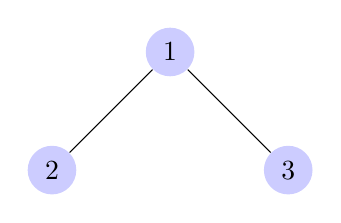
\begin{tikzpicture}
        \node[circle,fill=blue!20] (1) at (0,1.5) {1};
        \node[circle,fill=blue!20] (2) at (-1.5,0) {2};
        \node[circle,fill=blue!20] (3) at (1.5,0) {3};
        
        \draw (1) -- (2);
        \draw (1) -- (3);
        
    \end{tikzpicture}
    \caption{Grafo esempio.}
\end{figure}
 Il grafo presenta due massimi globali:
 \begin{align*}
     C_1 = \{1,2\} \qquad  x^{C_1} = (1 / 2, 1 / 2, 0) \\
     C_2 = \{1,3 \} \qquad x^{C_2} = (1 / 2, 0, 1 / 2)
 \end{align*}

Tuttavia come si evince dal seguente grafico, sono massimi globali anche tutti i punti del segmento $x'x''$ ovvero tutti i punti in $(1/2, \alpha / 2, (1 - \alpha) / 2) \, \forall \alpha \in [0,1]$.
\begin{figure}[h!]
    \centering
    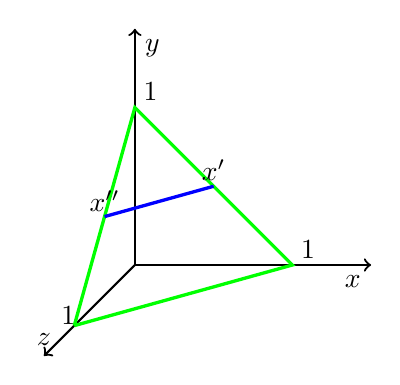
\begin{tikzpicture}[scale=2]
        %draw the main coordinate system axes
        \draw[thick,->] (0,0,0) -- (1.5,0,0) node[anchor=north east]{$x$};
        \draw[thick,->] (0,0,0) -- (0,1.5,0) node[anchor=north west]{$y$};
        \draw[thick,->] (0,0,0) -- (0,0,1.5) node[anchor=south]{$z$};
        
        \draw[thick, color=green, very thick] plot coordinates{(0,0,1) (0,1,0) (1,0,0) (0,0,1)};
        \draw[color=blue, very thick] (.5, .5, 0) -- (0,.5,.5);
        
        \node at (.5,.6,0) {$x'$};
        \node at (0,.6,.5) {$x''$};
        
        \node at (1.1,0.1,0) {1};
        \node at (0.1,1.1,0) {1};
        \node at (0,0.1,1.1) {1};
        
    \end{tikzpicture}
    \caption{Soluzioni spurie in MCP}
\end{figure}

Dunque $x'$ e $x''$ \textbf{non} sono vettori caratteristici e non possono essere utilizzati per la soluzione del MCP.

\newpage

Quello che è stato fatto finora è prendere il problema $P$ di clique massima nel discreto e trasformarlo in un problema $P'$ di ottimizzazione quadratica nel continuo. A questo punto è necessario mappare la soluzione del problema $P'$ in una soluzione del problema originale $P$.  Questo è possibile se la soluzione ottenuta in $P'$ è un vettore caratteristico.\\

Il problema delle soluzioni spurie è stato recentemente risolto da Bomze (1995) proponendo una versione regolarizzata di $f_G(x)$. La soluzione consiste nel sommare $1/2$ alla diagonale principale della matrice di adiacenza $A$.
\begin{align*}
    A' = A + \frac{1}{2} I
\end{align*}
Da cui si ottiene:
\begin{align*}
    \hat{f}_G(x) = x^T A' x = x^T \left( A + \frac{1}{2} I \right) x 
\end{align*}
Dove I è la matrice identità, ovvero una matrice quadrata dello stesso lato di $A$ con tutti gli elementi in diagonale principale ad 1 e tutti gli elementi al di fuori di essa a 0.\\


\begin{figure}[h!]
    \centering
    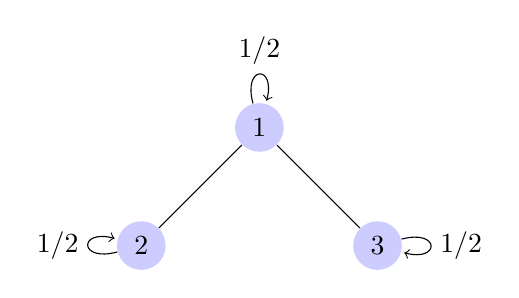
\begin{tikzpicture}
        \node[circle,fill=blue!20] (1) at (0,1.5) {1};
        \node[circle,fill=blue!20] (2) at (-1.5,0) {2};
        \node[circle,fill=blue!20] (3) at (1.5,0) {3};
        
        \path
		(1) edge (2)
		(1) edge (3)
		(1) edge[loop above] node{$1/2$} (1)
		(2) edge[loop left] node{$1/2$} (2)
		(3) edge[loop right] node{$1/2$} (3)
		;
        
    \end{tikzpicture}
    \caption{Soluzione problema delle soluzioni spurie (Bomze).}
\end{figure}

Riassumendo il problema della cricca massima dato un grafo $G = (V, E)$ è definito nel seguente modo:
\begin{align*}
	\max(\hat{f}_G(x)) \text{ tale che } x \in S_n
\end{align*}
Sia $C \subseteq V$ e sia $x^C$ il suo vettore caratteristico allora:
\begin{enumerate}
	\item $C$ è una clique massima di $G$ sse $x^C$ è un massimo globale di $\hat{f} \in S_n$;
	\item $C$ è una clique massimale di $G$ sse $x^C$ è un massimo locale di $\hat{f} \in S_n$;
	\item ogni massimo locale è un vettore caratteristico ed è locale stretto. 
\end{enumerate}

\newpage

Il risultato precedente garantisce che \emph{tutti} i massimizzatori di $\hat{f}$ su $S_n$ sono stretti, e sono sono vettori caratteristici di clique massima/massimale in un grafo. In particolare esiste una corrispondenza uno-a-uno da una parte tra le clique massimali e massimizzatori locali di $\hat{f}$ su $S_n$, dall'altra tra clique massima e massimizzatore globale.

% section problema_della_cricca_massima (end)


% chapter ottimizzazione_con_le_reti_neurali (end)
